\documentclass{beamer}

\usepackage[utf8]{inputenc}
\usepackage[T1]{fontenc}
\usepackage[ngerman]{babel}

\usepackage{multicol}

\usepackage{dsfont}

\usepackage{graphicx}

\usepackage{amsmath}
\usepackage{amssymb}
\usepackage{amsfonts}

\usepackage{microtype}
\usepackage{lmodern}

\usetheme{Goettingen}  %% Themenwahl
 
\title{Diffusion}
\author{Frederik Strothmann und Henrik Jürgens}
\date{\today}
 
\begin{document}
\maketitle
\frame{\tableofcontents[currentsection]}
 


\section{Generelles}

\begin{frame} %%Eine Folie
  \frametitle{Problemstellung} %%Folientitel
 \begin{itemize}
 		\item Diffusion in einem Kasten mit zwei Kammern
        \item N Teilchen
        \item Wechselwirkung durch zentralen Stoß
\end{itemize}
\end{frame}

\begin{frame} %%Eine Folie
  \frametitle{Motivation} %%Folientitel
 \begin{itemize}
 		\item Untersuchen von Verteilungsprozessen in Abhängigkeit von:
 		\begin{itemize}
 			\item Kastengröße
 			\item Spaltgröße
 			\item Anzahl/Größe/Masse der Teilchen
 		\end{itemize}
\end{itemize}
\end{frame}


\begin{frame} %%Eine Folie
  \frametitle{Aktueller Programm-Umfang} %%Folientitel
 \begin{itemize}
 		\item Kasten beliebig einstellbar
 		\item Teilchen automatisch generieren oder von Hand erstellbar
 		\item Plotten der Teilchen bahnen
 		\item Plotten der Teilchenanzahl pro Kammer gegen die Zeit
 		\item Plotten der Verteilung der Iterationsdauern
 		\item Auswertung der Iterationsdauern (Min,Max,Mittelwert)
\end{itemize}
\end{frame}



\section{Aufbau des Programms}

\begin{frame} %%Eine Folie
  \frametitle{UML-Diagramm} %%Folientitel
  \begin{figure}[htb]
		\centering
		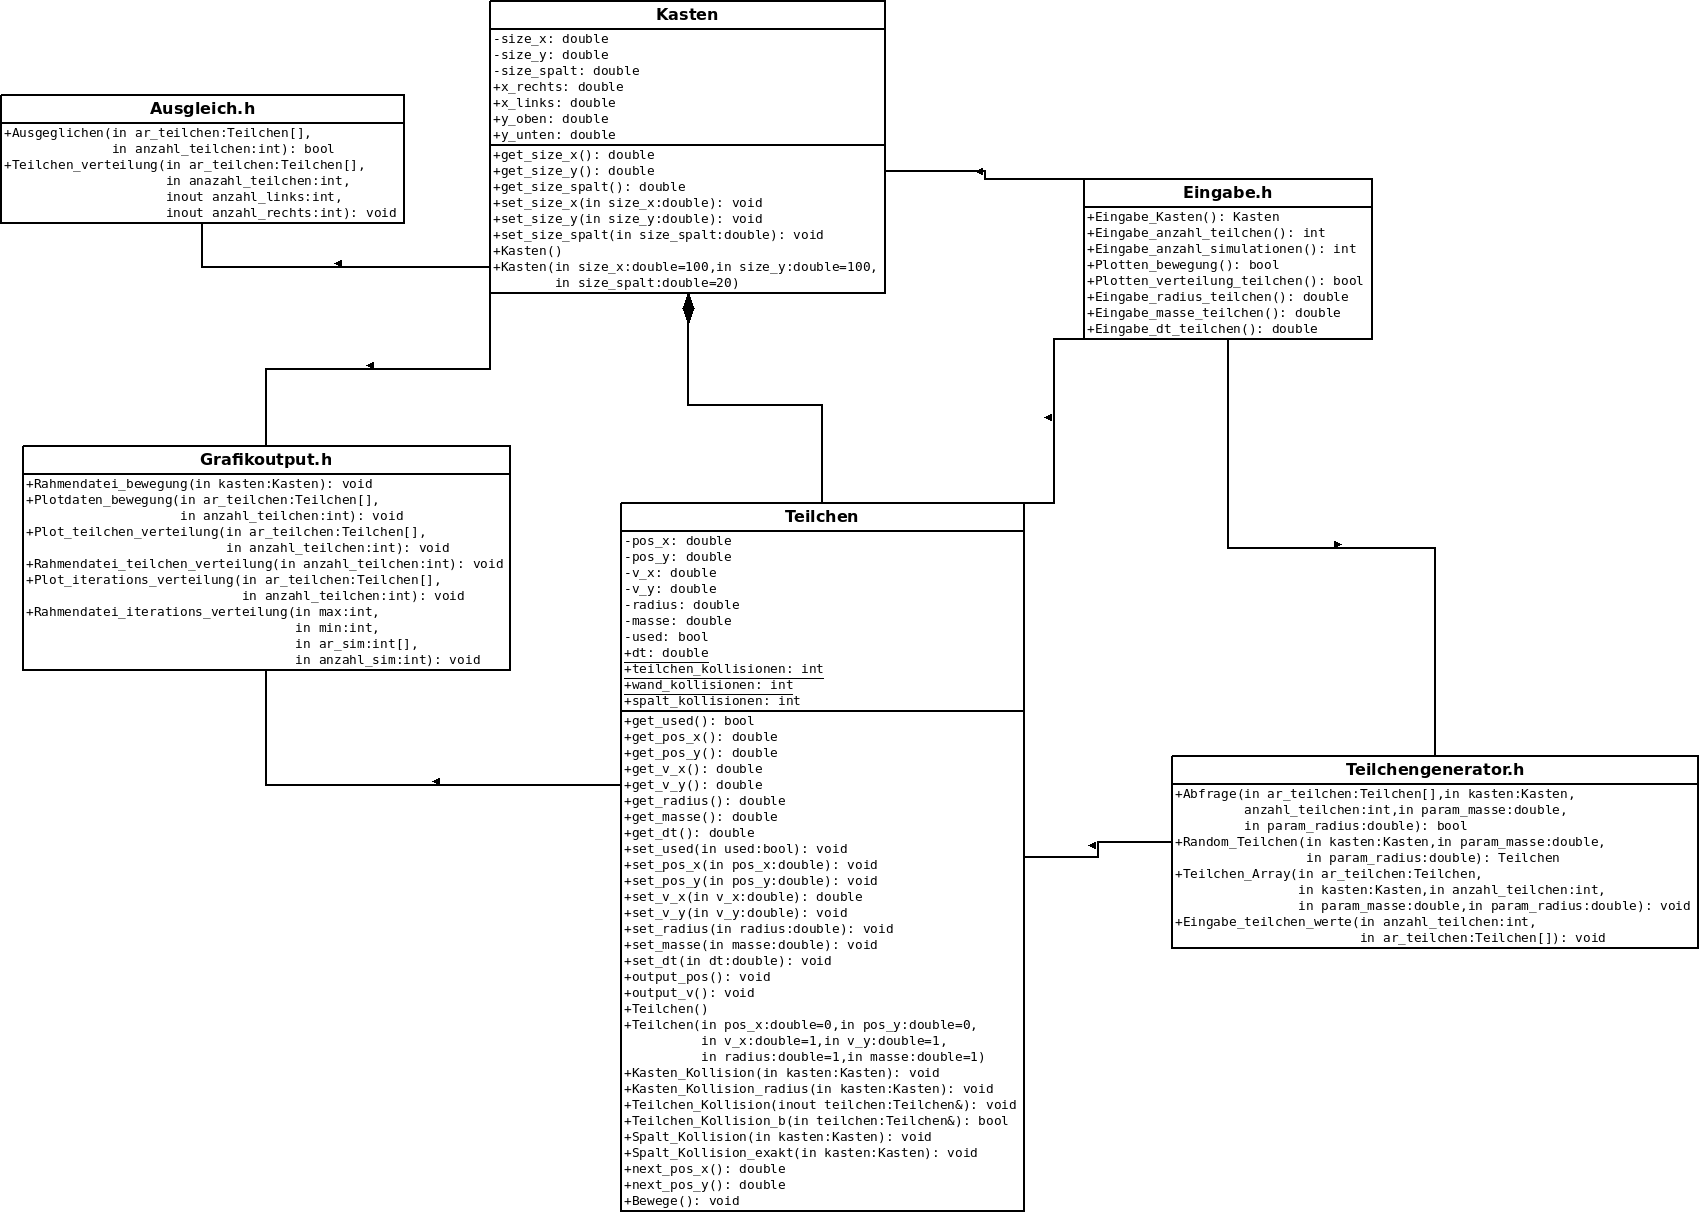
\includegraphics[scale = 0.17]{UML-Projekarbeit.png}
		\caption{UML-Diagramm des Programms}
  \end{figure}
\end{frame}

\begin{frame} %%Eine Folie
  \frametitle{Flussiagramm der main.cpp} %%Folientitel
  \begin{figure}[htb]
		\centering
		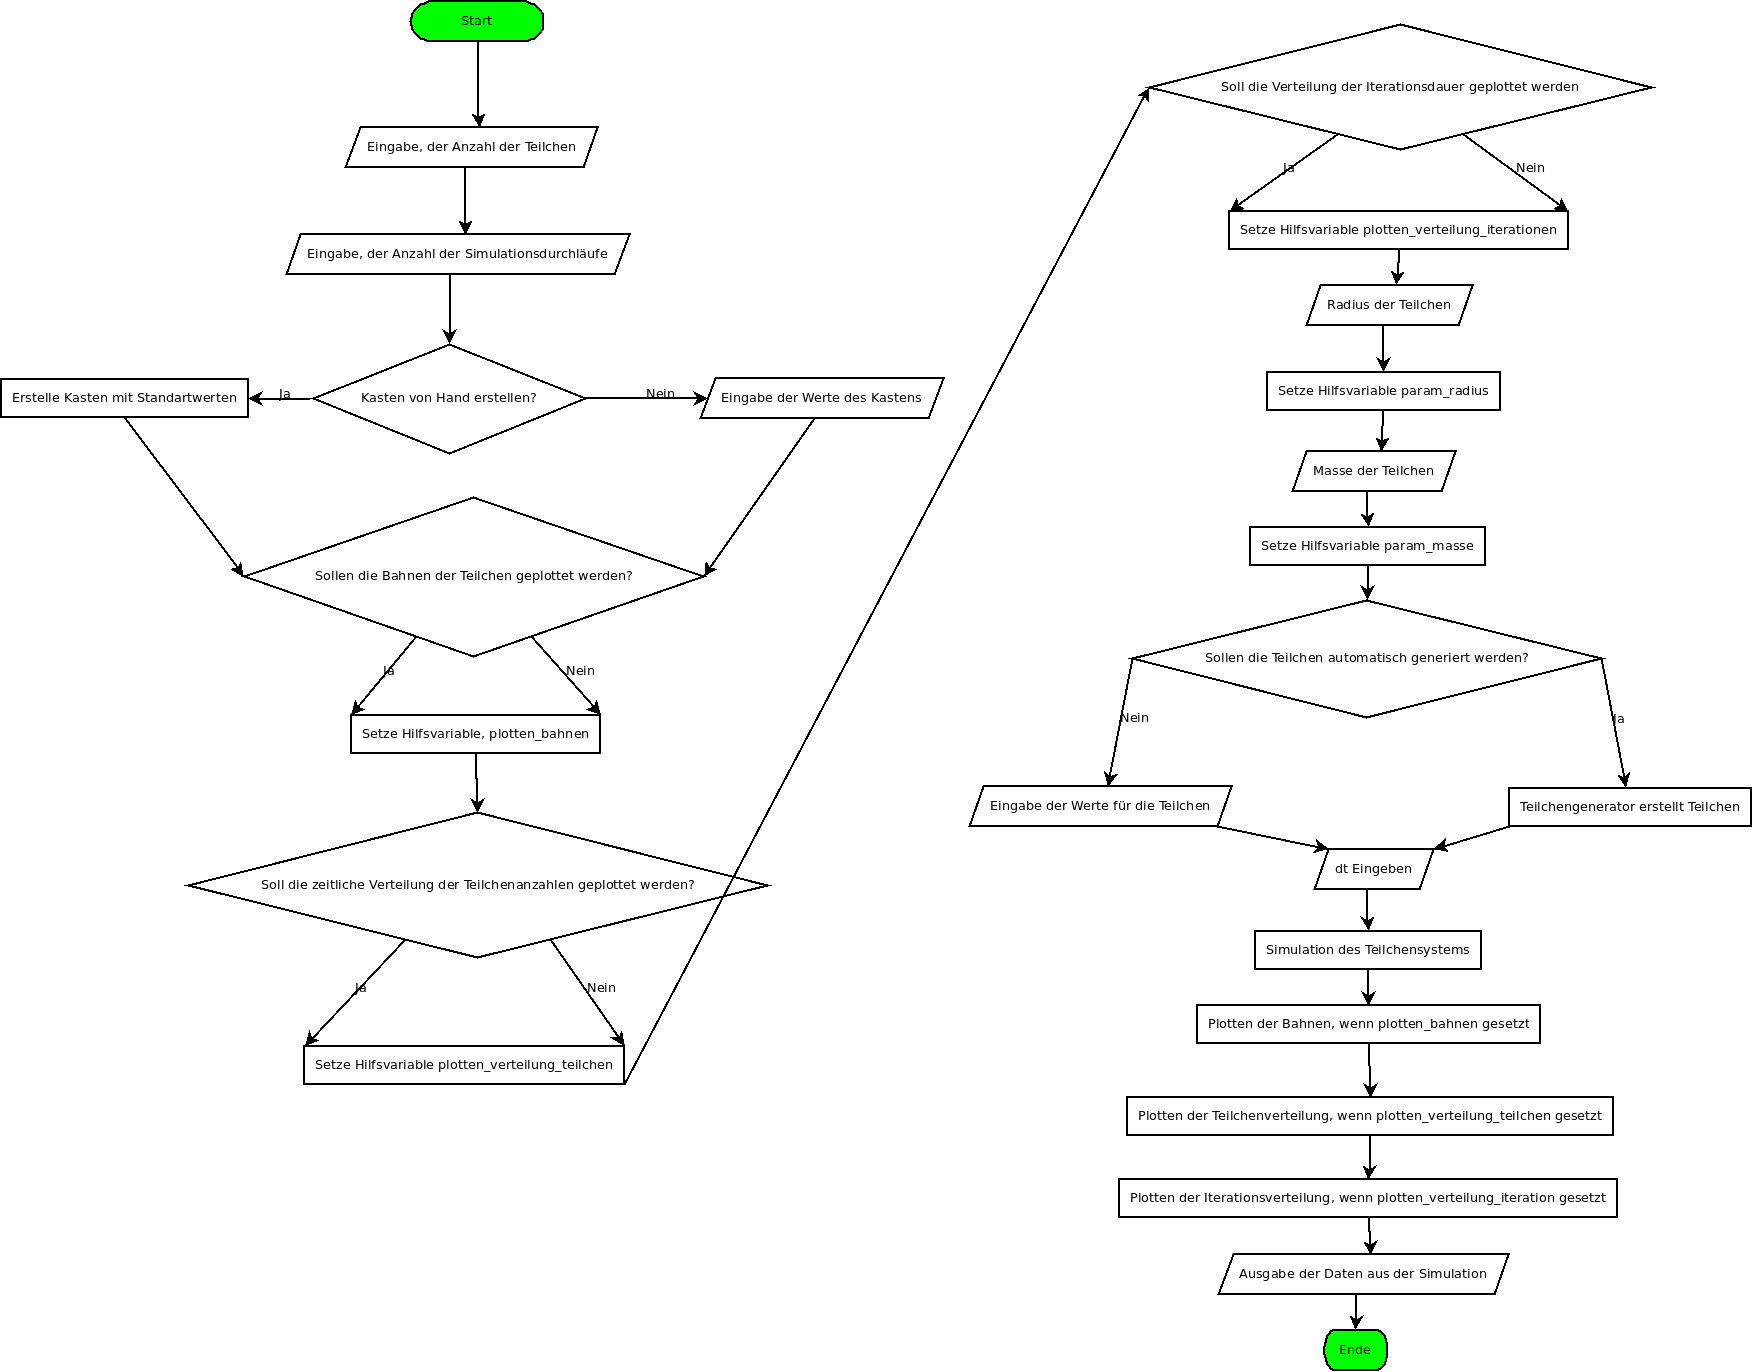
\includegraphics[scale = 0.16]{Flussdiagramm_main.png}
		\caption{Flussiagramm des Programms}
  \end{figure}
\end{frame}

\begin{frame} %%Eine Folie
  \frametitle{Kasten} %%Folientitel  
  \begin{figure}
		\centering
		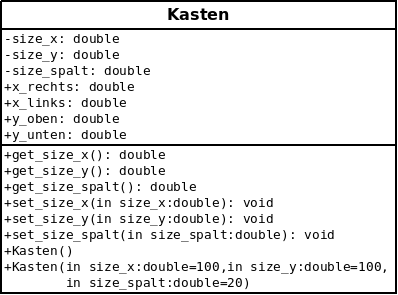
\includegraphics[scale = 0.27]{Kasten.png}
		\caption{Attribute und Methoden der Klasse Kasten}
  \end{figure}
  \begin{itemize}
  	\item Liefert Umgebung, für den Diffusionsprozess
  \end{itemize}
\end{frame}

\begin{frame} %%Eine Folie
	  \frametitle{Kasten} %%Folientitel  
 \begin{figure}
		\centering
		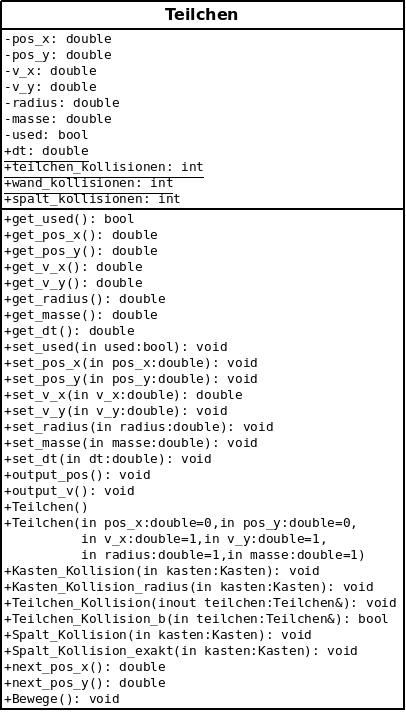
\includegraphics[scale = 0.2]{Teilchen.png}
		\caption{Attribute und Methoden der Klasse Teilchen}
  \end{figure}
  	\begin{itemize}
	  	\item Liefert Teilchen, mit denen der Diffusionsprozess untersucht wird
	 	\item Beinhaltet die gesamte Kollisions und Bewegungsberechnung
	\end{itemize}
\end{frame}

\begin{frame} %%Eine Folie
  \frametitle{Eingabe.h} %%Folientitel  
  \begin{figure}
		\centering
		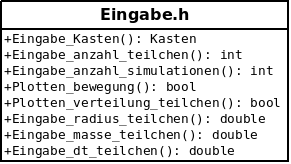
\includegraphics[scale = 0.27]{Eingaben.png}
		\caption{Funktion für die Eingabe}
  \end{figure}
  \begin{itemize}
  	\item Liefert Eingabeinterface
  \end{itemize}
\end{frame}

\begin{frame} %%Eine Folie
  \frametitle{Teilchengenerator.h} %%Folientitel  
  \begin{figure}
		\centering
		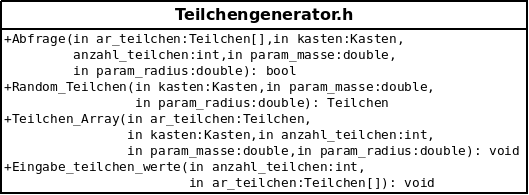
\includegraphics[scale = 0.27]{Teilchengenerator.png}
		\caption{Funktionen zum erstellen der Teilchen}
  \end{figure}
  \begin{itemize}
  	\item Liefert Funktionen zum automatischen und händischen generieren der Teilchen
  \end{itemize}
\end{frame}

\begin{frame} %%Eine Folie
  \frametitle{Ausgleich.h} %%Folientitel  
  \begin{figure}
		\centering
		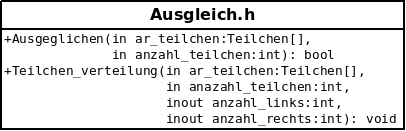
\includegraphics[scale = 0.27]{Ausgleich.png}
		\caption{Funktionen zum feststellen, ob sich ein Gleichgewichtszustand eingestellt hat}
  \end{figure}
  \begin{itemize}
  	\item Prüft, ob der Diffusionsprozess abgeschlossen ist
  \end{itemize}
\end{frame}

\begin{frame} %%Eine Folie
  \frametitle{Grafikoutput.h} %%Folientitel  
  \begin{figure}
		\centering
		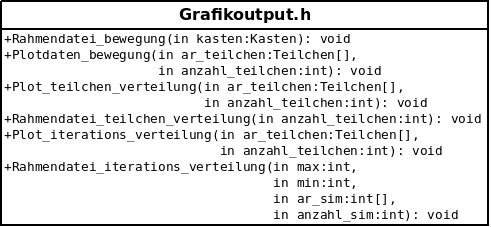
\includegraphics[scale = 0.27]{Grafikoutput.png}
		\caption{Funkionen zum darstellen der Simulationsergebnisse}
  \end{figure}
  \begin{itemize}
  	\item Liefert Funktionen um die Daten aus der Simulation Grafisch darzustellen
  \end{itemize}
\end{frame}

\end{document}